% !TEX encoding = UTF-8 Unicode
\documentclass[titlepage,english,a4]{thesis}

\usepackage[nottoc,notlot,notlof]{tocbibind}
\usepackage[toc,page]{appendix}

\setlength{\cftbeforeloftitleskip}{5pt} % LOF: Listing of Figures
\setlength{\cftbeforelottitleskip}{5pt} % LOT: Listing of Tables

\usepackage{kantlipsum}
\setlength{\textheight}{10in}%

\usepackage{blindtext}
\usepackage{tocbibind}
\usepackage{hyperref}


\def\DATE{\today}
\def\TITLE{Thesis title}
\def\SUBHEADING{A example on a Thesis}
\def\AUTHOR{Elias Korhonen}
\def\LEVEL{Master's Thesis}
\def\PROGRAMME{Master of Engineering - Big Data Analytics}
\def\UNIVERSITY{Arcada University of Applied Sciences}
\def\IDENTIFICATION{313}
\def\SUPERVISOR{Ludwig Von Drake}
\def\COMMISSIONEDBY{Scrooge McDuck}
\def\KEYWORDS{Ducks Birds Hawks}
\def\PAGECOUNT{ \pageref{LastPage} }
\def\DATEACCEPTANCE{1.10.2054}

\begin{document}

\begin{titlepage}
\maketitle
\end{titlepage}

\begin{abstract}{english}
This is the abstract. Blah blah blah...
\end{abstract}


%\begin{abstract}{swedish}
%Ett sammandrag på svenska bokstaven där bokstäverna  å , ä och ö är inkluderade.
%Check that the encoding is correct so that åäö are visible.
%\end{abstract}

%\begin{abstract}{finnish}
%Samma på finska
%\end{abstract}

% Remove for swedish
%\renewcommand{\contentsname}{INNEHÅLL}
%\renewcommand{\listfigurename}{FIGURER}
%\renewcommand{\listtablename}{TABELLER}



\tableofcontents
\addtocontents{toc}{\vspace{0.5cm}}

\listoffigures
\addtocontents{lof}{\vspace{0.5cm}}

\listoftables
\addtocontents{lot}{\vspace{0.5cm}}

\cleardoublepage

\section*{Foreword}
\kant[11]

\cleardoublepage

\section{Introduction}
This is in the Introduction
\subsection{Background}
Go back to the underlining problem about Ducks
\subsubsection{More about the background}
You can find more info about Donald Ducks at wikipedia \citep{swasey2015silver}


\subsubsection{How to cite}

\begin{verbatim}
 %   \cite{key} ==>>                Jones et al. (1990)
 %   \citet*{key} ==>>               Jones, Baker, and Smith (1990)
 %   \citep{key} ==>>                (Jones et al., 1990)
 %   \citep*{key} ==>>               (Jones, Baker, and Smith, 1990)
 %   \citep[chap. 2]{key} ==>>       (Jones et al., 1990, chap. 2)
 %   \citep[e.g.][]{key} ==>>        (e.g. Jones et al., 1990)
 %   \citep[e.g.][p. 32]{key} ==>>   (e.g. Jones et al., p. 32)
 %   \citeauthor{key} ==>>           Jones et al.
 %   \citeauthor*{key} ==>>          Jones, Baker, and Smith
 %   \citeyear{key} ==>>             1990
\end{verbatim}

\subsection{Some random subsection}
\kant[1]

\subsection{Another random subsection}
\kant[2]
\cleardoublepage

\section{Related Work}

Many authors have worked in the same area~\citep*{leal2015optimizing}. In special,  \citeauthor{espinosa2019reinforcement} have discussed more in detail.

\kant[3-5]

\begin{figure}
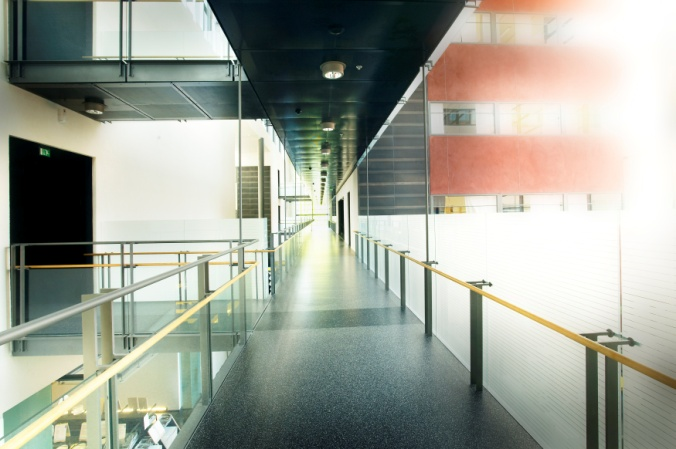
\includegraphics[width=8cm]{figures/arcada.jpg}
\caption{The interior of Arcada. Photograph Valtteri Kantanen Arcada 2008}
\end{figure}

\kant[2]

\cleardoublepage

\section{Research Methodology}

\kant[7-11]

\begin{table}
 \caption{An example of a table}
\begin{tabular}{ |p{3cm}||p{3cm}|p{3cm}|p{3cm}|  }
 \hline
 \multicolumn{4}{|c|}{Country List} \\
 \hline
 Country Name     or Area Name& ISO ALPHA 2 Code &ISO ALPHA 3 Code&ISO numeric Code\\
 \hline
 Afghanistan   & AF    &AFG&   004\\
 Aland Islands&   AX  & ALA   &248\\
 Albania &AL & ALB&  008\\
 Algeria    &DZ & DZA&  012\\
 American Samoa&   AS  & ASM&016\\
 Andorra& AD  & AND   &020\\
 Angola& AO  & AGO&024\\
 \hline
\end{tabular}
\end{table}


\cleardoublepage

\section{Experiments}

I like Donald Duck, in \cite{leal2018web}

Here another reference like in \cite*{leal2018web}
\cleardoublepage

\section{Results}

I like Donald Duck, in \cite{leal2018web}

Here another reference like in \cite*{leal2018web}

\cleardoublepage
\section{Conclusions}
\kant[10]



% Here the bibliography
\cleardoublepage
\phantomsection
% Uncomment for swedish
%\renewcommand{\bibname}{Källor}
\renewcommand{\bibname}{References}
\bibliographystyle{bibliography}
\bibliography{7-references}



%\renewcommand{\bibname}{References}
%\bibliographystyle{bibliography}
%\bibliography{7-references}
%\newpage
\cleardoublepage
\phantomsection
\addcontentsline{toc}{section}{Appendix A}
\section*{Appendix A}
\kant[21]


\addcontentsline{toc}{section}{Appendix B}
\section*{Appendix B}
\kant[22]



\end{document} 
